\documentclass{article}
\usepackage[english]{babel}
\usepackage[a4paper, left=3.5cm, right=3.5cm, top=3cm, bottom=4cm]{geometry}
\usepackage{graphicx} % Required for inserting images
\usepackage{tcolorbox}
\usepackage{booktabs} % For nicer tables
\usepackage[hidelinks]{hyperref}
\usepackage{ffcode}
\usepackage{todonotes}
\usepackage[dvipsnames]{xcolor}

\font\myfont=cmr10 at 28pt
\setlength{\parindent}{0pt}

\hypersetup{
    colorlinks=true,
    linkcolor=NavyBlue,
    filecolor=Blue,      
    urlcolor=NavyBlue,
    citecolor=NavyBlue,
    pdftitle={WiFind: Indoor localization through WiFi fingerprinting},
    pdfpagemode=FullScreen,
    }
\bibliographystyle{IEEEtran}

\title{{\myfont WiFind}}
\author{
    Gabriele Aprile
    \and
    Matteo Cardellini
    \and
    Andreea Scrob
}
\date{March 2025}

\begin{document}

\maketitle

\begingroup
\hypersetup{hidelinks} 
\tableofcontents
\endgroup

\newpage

%%%%%%%%%%%%%%%%%%%%%%%%
\section{Introduction}
User localization inside buildings is an important problem in many domains, such as security, home automation, and indoor navigation. One of the most widely used techniques to determine a user's position is \textbf{WiFi fingerprinting}\footnote{A localization technique based on collecting and analyzing the "fingerprints" of WiFi signals in a given area. Each location has a unique \textit{signature} produced by the combination of signals received from multiple access points, which is then used to estimate the user's position.}, which leverages the received signal strength (RSSI\footnote{\textit{Received Signal Strength Indicator} denotes the power of the signal received by a device, measured in dBm (decibels relative to 1 mW).}) from several access points and employs machine learning models to estimate position.

\subsection{Problem description}
The problem addressed here is to determine, as precisely as possible, the location of a user in an indoor environment using only network data, avoiding extra hardware such as GPS or external sensors.\\
In our case, the objective is to \textit{identify which room of the Computer Science Department a given user is located in}, based solely on information from AlmaWiFi access points.

\subsection{Proposed solutions}
To tackle the problem we propose to:
\begin{itemize}
    \item select a well-defined building area and collect data within it to \textbf{construct a dataset};
    \item \textbf{choose a simple and effective machine learning model}, such as \textit{K-Nearest Neighbors (KNN)} or \textit{Random Forest}, to classify locations;
    \item \textbf{evaluate relevant metrics} and \textbf{tune the model} to achieve satisfactory performance.
\end{itemize}

\section{Proposed methods}
\subsection{Dataset}
\subsubsection{Collection and preprocessing}
\begin{figure}[ht!]
    \centering
    {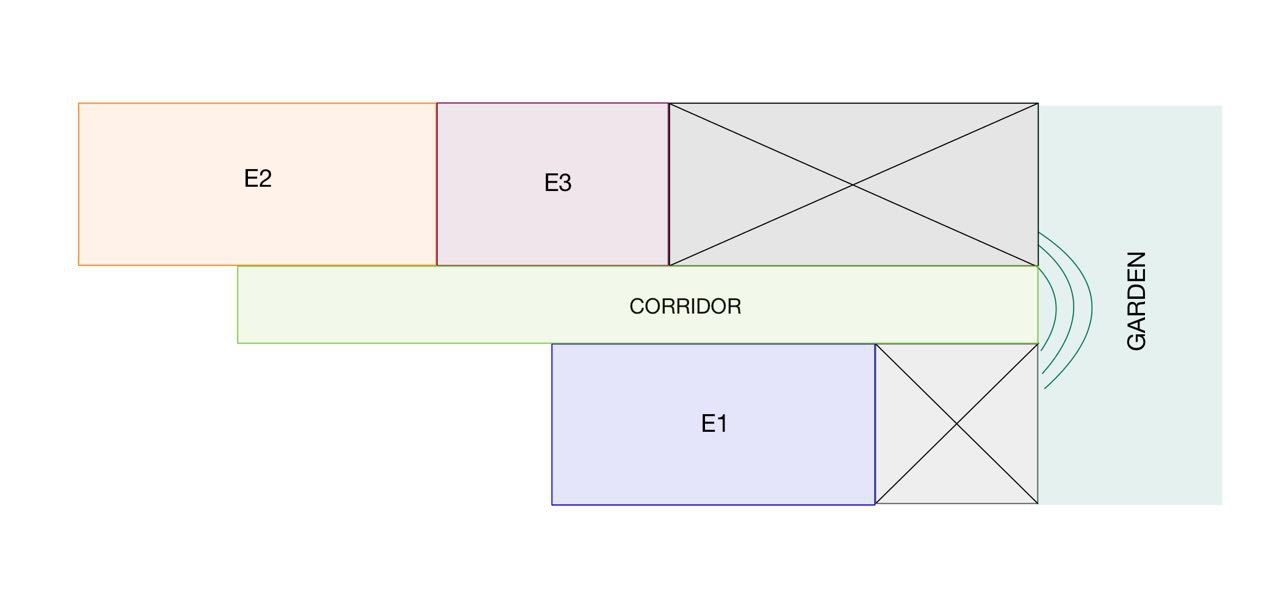
\includegraphics[scale=0.28]{img/piantinaErcolani.JPG}}
    \caption{Map of the Ercolani building with the rooms used for data collection}
    \label{Pianta}
\end{figure}
We created a project-specific \textbf{dataset} by collecting measurements from the various \textit{access points} in the Ercolani building (map shown in \autoref{Pianta}) using a set of Python scripts.
To evaluate the impact of obstacles on radio propagation, which can cause interference, measurements were taken twice for each room: once with the room empty (\textit{Empty}) and once with the room crowded (\textit{Crowded}).\\
After collection, data were filtered to keep only records related to the \textbf{AlmaWIFI} network, as shown in \autoref{tab:wifi_data}.

\begin{table}[ht!]
    \centering
    \small
    \begin{tabular}{llc c c cc}
        	oprule
        Room & Condition & AP1 & AP2 & \dots & AP41 & AP42 \\
        \midrule
        E1 & Empty & -76.0 &  & \dots & -89.0 & \\

        E2 & Empty & -45.0 & -66.0  & \dots &  & \\
        E3 & Empty & -64.0 & -79.0 & \dots &  &  \\
        Corridor & Empty & -48.0 & -66.0  & \dots &  & \\
        Garden & Empty &  &   & \dots &  & -91.0 \\
         \vdots & \vdots & \vdots & \vdots & \vdots & \vdots & \vdots \\
        E1 & Crowded & -84.0 &  & \dots & -91.0 &  \\
        E2 & Crowded & -47.0 & -64.0  & \dots &  & \\
        E3 & Crowded & -66.0 & -78.0 & \dots &  &  \\
        Corridor & Crowded &  & -93.0  & \dots &  & \\
        Garden & Crowded & -78.0 &   & \dots &  & \\

        \bottomrule
    \end{tabular}
    \caption{Excerpt of the dataset \textit{wifi\_fingerprinting\_dataset\_raw.csv}}
    \label{tab:wifi_data}
\end{table}

\subsubsection{Exploratory data analysis}
Using plots, we conducted preliminary analyses on the collected data.\\
In particular, we produced a \textbf{histogram} showing the total number of detections for each access point (AP) (see \autoref{FreqAP}).
We also generated a \textbf{heatmap} (\autoref{heatmap}) of Wi\-Fi signal strength that highlights the average intensity recorded for each AP across different areas (E1, E2, E3, Corridor, Garden) and the two environmental conditions (Empty, Crowded). The colours in the heatmap visually represent the received signal strength.\\
These plots clarified the dataset structure and revealed that some APs were not very informative (few detections), suggesting further cleaning and feature selection were needed.

\begin{figure}[ht!]
    \centering
    {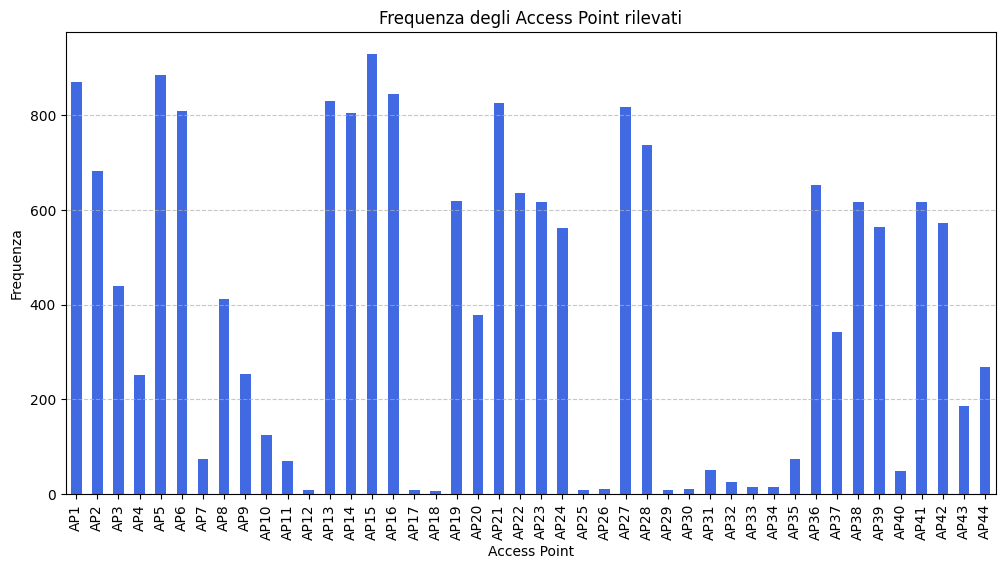
\includegraphics[scale=0.50]{img/output.png}}
    \caption{Histogram of total detections per Access Point (AP)}
    \label{FreqAP}
\end{figure}

\begin{figure}[ht!]
    \centering
    {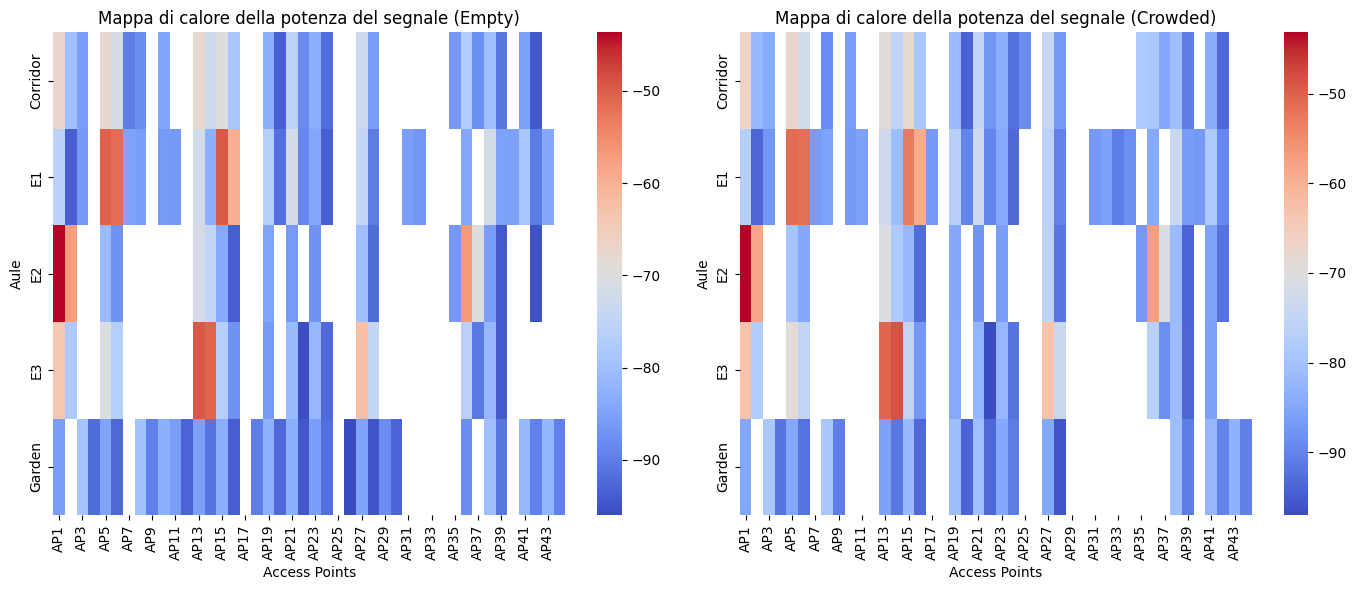
\includegraphics[scale=0.38]{img/ColorMap.png}}
    \caption{Heatmap of average Wi\-Fi signal strength in \textit{Empty} and \textit{Crowded} conditions}
    \label{heatmap}
\end{figure}

\subsubsection{Dataset manipulations}
As previously noted, some APs were detected far less frequently than others (\autoref{FreqAP}). To address this, we \textbf{reduced the presence of under-represented APs} by removing any AP with fewer than 400 detections using a Python script. The resulting dataset is called \textbf{cut400}.\\
This step also made the dataset more "tall" (fewer features relative to the number of instances), reducing the risk of high-dimensional feature space issues that can hurt models such as KNN.\\
We created additional variants: a normalized dataset and a binarized dataset.\\
In the \textbf{normalized} dataset, each RSSI value was scaled to the range [0,1] using Min–Max normalization:
\[X_{norm}= \frac{X-X_{min}}{X_{max}-X_{min}}\]
In the \textbf{binarized} dataset, values indicate only signal presence or absence: \textbf{1} for presence and \textbf{0} for absence. An excerpt is shown in \autoref{tab:wifi_data_bin}.\\

\begin{table}[ht!]
    \centering
    \small
    \begin{tabular}{llc c c cc}
        	oprule
        Room & Condition & AP1 & AP2 & \dots & AP41 & AP42 \\
        \midrule
        E1 & Empty & 1 & 0 & \dots & 1 & 0 \\
        E2 & Empty & 1 & 1  & \dots & 0 & 0\\
        E3 & Empty & 1 & 1 & \dots & 0 & 0 \\
        Corridor & Empty & 1 & 1  & \dots & 0 &0 \\
        Garden & Empty & 0 & 0  & \dots &  0& 1\\
         \vdots & \vdots & \vdots & \vdots & \vdots & \vdots & \vdots \\
        E1 & Crowded & 1 & 0 & \dots & 1 & 0 \\
        E2 & Crowded & 1 & 1  & \dots & 0 & 0\\   
        E3 & Crowded & 1 & 1 & \dots & 0 & 0 \\
        Corridor & Crowded & 0 & 1  & \dots & 0 & 0\\
        Garden & Crowded & 1 & 0  & \dots & 0 & 0\\
        \bottomrule
    \end{tabular}
    \caption{Excerpt of the file \textit{wifi\_fingerprinting\_dataset\_binarized.csv}}
    \label{tab:wifi_data_bin}
\end{table}

To make \textit{cut400} compatible with model training, missing values were replaced with \textbf{-200}, a synthetic value representing "an access point too far to be detected." This substitution is not applied to the \textit{binarized} and \textit{normalized} variants, which by construction contain values for all fields.

Further discussion about the use of these alternative datasets appears later.

\begin{figure}[ht!]
    \centering
    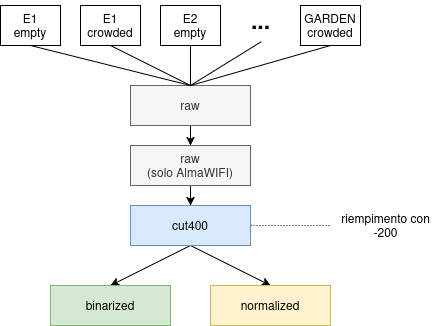
\includegraphics[width=0.5\linewidth]{img/datasetHistory.png}
    \caption{Dataset evolution diagram: from raw to cut400, normalized and binarized}
    \label{fig:datasetHistory}
\end{figure}


\subsection{Models}
We followed a methodological approach grounded in our academic background to structure the work rigorously.\\

Since the task is a \textbf{classification} problem, we started with a K-Nearest Neighbors (\textbf{KNN}) implementation as a simple, well-known baseline. KNN is a supervised algorithm based on proximity: it assigns a label to a new sample based on the majority label among its \textbf{k} nearest neighbors according to a chosen distance metric. This baseline provides a reference for evaluating later, more sophisticated approaches.\\
We also experimented with more advanced algorithms such as Random Forest.

In the literature we found a relevant paper \cite{Shang2022} that compares several machine learning methods for WiFi fingerprinting. It highlights the trade-offs of different approaches, for example:
\begin{itemize}
    \item \textbf{KNN}: well-suited for moderate-sized datasets and easy to implement and tune; less recommended when the number of features becomes very large.
    \item \textbf{SVM}: effective in high-dimensional spaces by finding separating hyperplanes; can be sensitive to outliers and overlapping classes.
    \item \textbf{Random Forest}: robust and generalizes well for large datasets; as an ensemble of decision trees it reduces overfitting and yields stable predictions.
\end{itemize}

Since our datasets are moderate in size and the feature count never exceeds 44 (maximum number of detected APs), we focused on KNN and hyperparameter tuning. If KNN proved insufficient, we planned to explore other classifiers more deeply.

%%%%%
\subsection{K-Nearest Neighbors}
\subsubsection{Dataset splitting}
To evaluate robustness under different crowding conditions, we created three dataframes corresponding to \textbf{Empty} (room empty), \textbf{Crowded} (room crowded) and \textbf{Hybrid} (combined) scenarios.\\
We defined a \textit{split\_data} function that splits each subset into a \textbf{training set} (70\%) and a \textbf{test set} (30\%) using stratified sampling to preserve class proportions. No explicit validation set was created; validation is performed with the technique described next.

\subsubsection{Model optimization}
While researching KNN improvements we considered approaches from the literature such as Weighted KNN (WKNN) \cite{electro}, which uses distance-based weighting to improve neighbor selection.\\
We chose a well-established approach: \textbf{Grid Search} to systematically find optimal hyperparameters.

    	extbf{Grid Search: searching for optimal hyperparameters}\\
Grid Search finds the best combination of \textbf{hyperparameters}\footnote{Parameters not learned by the model but set before training.} by exhaustively evaluating configurations.
The process consists of:
\begin{enumerate}
    \item defining a grid of possible values for each hyperparameter;
    \item training the model on every combination in the grid;
    \item evaluating each combination with a chosen metric (e.g. accuracy) and selecting the best.
\end{enumerate}

The grid we explored is shown in \autoref{tab:param_grid}.

\begin{table}[ht!]
\centering
\begin{tabular}{ll}
    	oprule
    	extbf{Parameter} & \textbf{Values explored} \\
    \midrule
    	exttt{n\_neighbors} & 3--19 \\
    	exttt{weights} & \texttt{['uniform', 'distance']} \\
    	exttt{algorithm} & \texttt{['ball\_tree', 'brute']} \\
    	exttt{metric} & \texttt{['euclidean', 'manhattan']} \\
    \bottomrule
\end{tabular}
\caption{Grid of values explored via Grid Search}
\label{tab:param_grid}
\end{table}

Overview of optimized parameters:
\begin{itemize}
    \item \textbf{n\_neighbors}: the $K$ value in KNN. Too small may overfit; too large may underfit. The range 3--19 was chosen as a practical compromise.
    \item \textbf{weights}: either \textit{uniform} (equal vote) or \textit{distance} (closer neighbors weighted more). Both were tested.
    \item \textbf{algorithm}: neighbor search method (\textit{ball\_tree}, \textit{brute}). Given the dataset size, \textit{ball\_tree} and \textit{brute} were appropriate choices.
    \item \textbf{metric}: distance metric (\textit{euclidean}, \textit{manhattan}). Both were evaluated.
\end{itemize}

Other hyperparameters (e.g. \textbf{p}, \textbf{leaf\_size}) were left at default values as they were considered less influential.

    	extbf{Cross Validation: robust validation of hyperparameter choices}\\
Grid Search was implemented using Scikit-Learn's \textit{GridSearchCV}, which evaluates each hyperparameter combination with \textbf{Cross Validation}. Training data are split into K folds; each iteration trains on K-1 folds and validates on the remaining fold. We used Stratified K-Fold to preserve class proportions. The mean performance across folds provides a stable estimate for selecting the best configuration.

\subsubsection{Evaluation metrics}
After selecting the best hyperparameters, model performance was evaluated using:
\begin{itemize}
    \item \textbf{Accuracy}: fraction of correctly classified instances.
    \item \textbf{Precision}: fraction of correct positive predictions among all positive predictions.
    \item \textbf{Recall}: fraction of true positives correctly identified.
    \item \textbf{F1-score}: harmonic mean of Precision and Recall.
\end{itemize}


%%%%%%%%%%%%%%%%%%%%%%
\section{Results and discussion}
After testing on different dataset variants, we found the \textbf{binarized} dataset (presence/absence) to be the most informative for our experiments compared to datasets with raw RSSI values.

This choice was motivated by suspected \textit{overfitting} when training on precise RSSI values: with a relatively small dataset, models may learn overly specific patterns, reducing generalization. Binarization improves generalization and makes results easier to interpret.

\subsection{Training}
Using GridSearchCV we found the best hyperparameters for each of the three scenarios (Empty, Crowded, Hybrid), reported in \autoref{tab:best_params}.\\
\begin{table}[ht!]
    \centering
    \begin{tabular}{ c c c c c c}
        \hline
        	extbf{Scenario} & \textbf{Algorithm} & \textbf{Metric} & \textbf{Neighbors} & \textbf{Weights} & \textbf{Best Accuracy} \\
        \hline
        Empty   & brute         & manhattan & 6  & distance & 0.9793  \\
        Crowded & ball\_tree    & manhattan & 15 & distance & 0.9340    \\
        Hybrid  & brute         & euclidean & 16 & uniform  & 0.9302     \\
        \hline
    \end{tabular}
    \caption{Optimal KNN configurations for the three scenarios, with corresponding accuracies}
    \label{tab:best_params}
\end{table}

For two scenarios the \textit{brute} algorithm was selected, reflecting that the dataset size allows exhaustive distance computation. The \textit{manhattan} metric was chosen in two cases, indicating a tendency to benefit from Manhattan distances in this feature space. The models were trained using these parameters.

\subsection{Testing}
We evaluated each trained model across all combinations of training and testing scenarios; results are shown in \autoref{tab:model_metrics}.
\begin{table}[ht!]
    \centering

    \begin{tabular}{c c c c c c }
        \hline
         	extbf{Train Model} & \textbf{Test Model} & Accuracy & Precision & Recall & F1-score \\
        \hline
        Empty   & Empty   & 0.932 & 0.935 & 0.932 & 0.931 \\
        Empty   & Crowded & 0.813 & 0.808 & 0.813 & 0.797 \\
        Empty   & Hybrid  & 0.912 & 0.912 & 0.912 & 0.909 \\
        Crowded & Empty   & 0.904 & 0.913 & 0.904 & 0.904 \\
        Crowded & Crowded & 0.887 & 0.884 & 0.887 & 0.884 \\
        Crowded & Hybrid  & 0.919 & 0.922 & 0.919 & 0.919 \\
        Hybrid  & Empty   & 0.959 & 0.962 & 0.959 & 0.959 \\
        Hybrid  & Crowded & 0.907 & 0.905 & 0.907 & 0.905 \\
        Hybrid  & Hybrid  & 0.929 & 0.933 & 0.929 & 0.929 \\
        \hline
    \end{tabular}
    \caption{KNN model evaluation: metrics for all training/testing combinations}
    \label{tab:model_metrics}
\end{table}

\begin{figure}[ht!]
    \centering
    {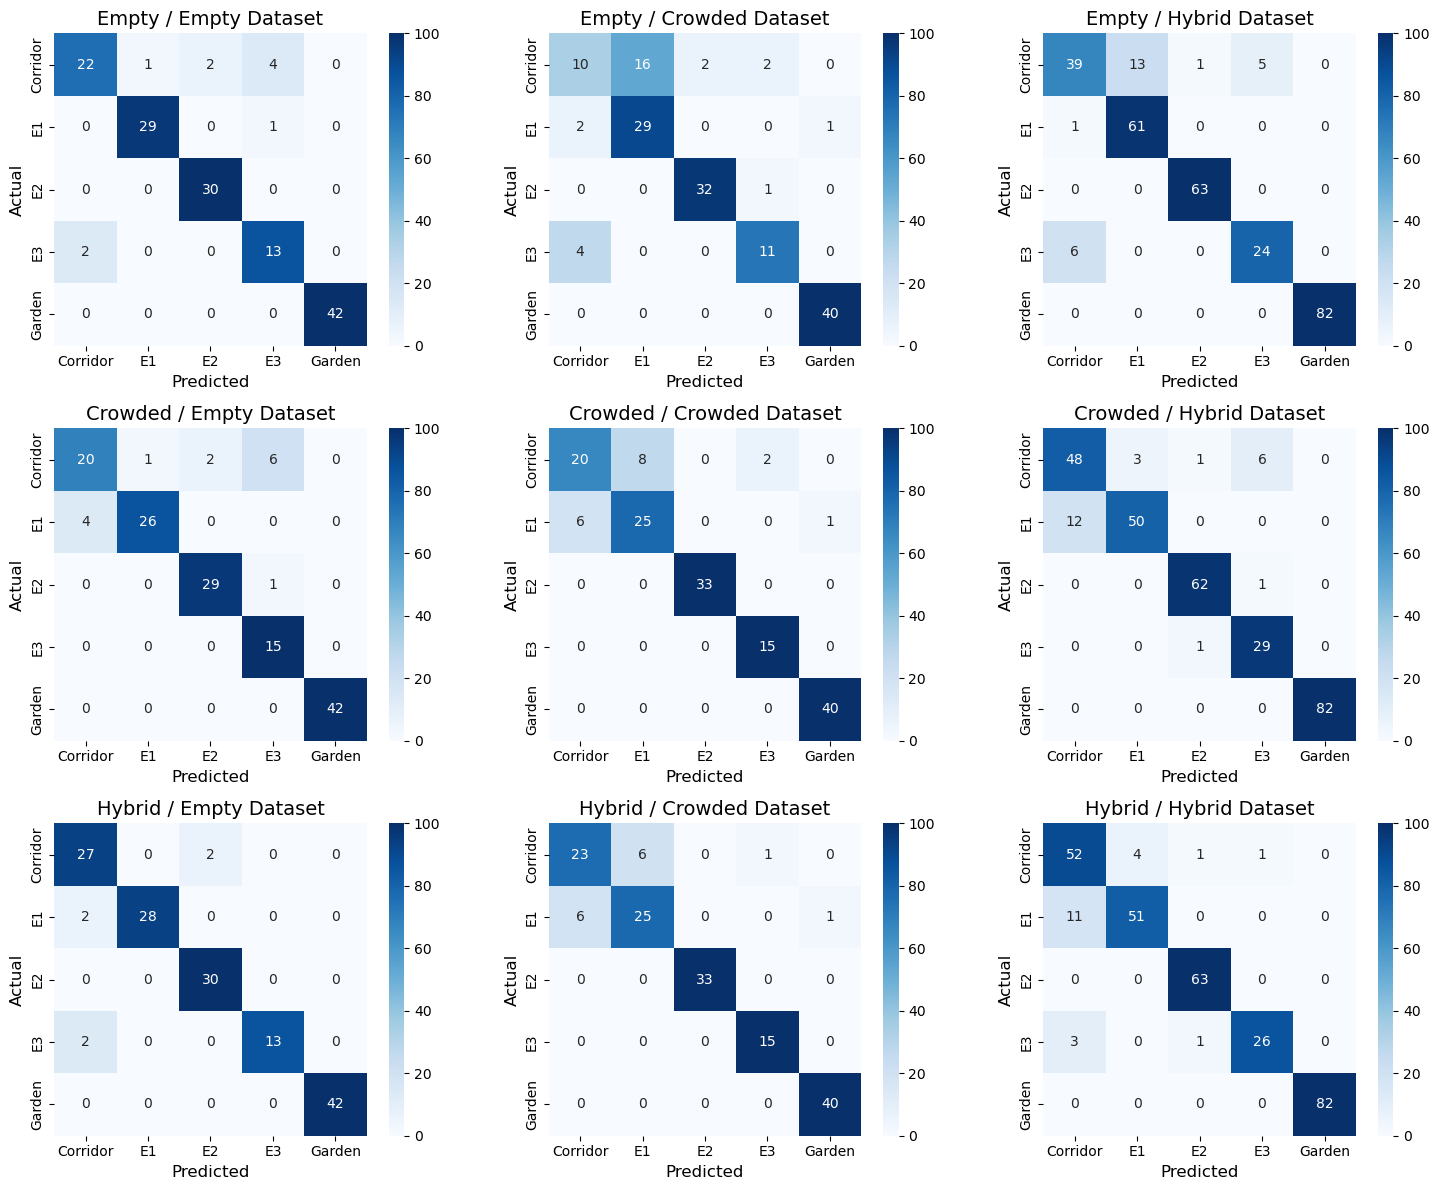
\includegraphics[scale=0.39]{img/MCGSCV.png}}
    \caption{Confusion matrices obtained from the optimized KNN model (GridSearchCV) on the \textit{binarized} dataset}
    \label{MCGtid}
\end{figure} 

From the confusion matrices in \autoref{MCGtid} and the metrics in \autoref{tab:model_metrics}, the model generally performs \textbf{better when training and test datasets match}, with an exception: the \textit{Crowded--Crowded} case is the worst performing, showing lower accuracy even compared to some cross-scenario evaluations.\\
The \textit{Hybrid} dataset proved the most adaptable since it trains on all conditions and yields globally better classification performance.\\

Overall, crowd presence does not appear to be a decisive factor for localization accuracy, although it introduces additional variability and noise.\\
The most frequent errors occur between \textbf{"Corridor" and "E1"}, which share the largest common area (\autoref{Pianta}); overlapping router coverage likely causes confusion. The \textbf{"Garden"} area is correctly classified in most cases due to its spatial separation from other rooms.

\section{Conclusion}
This study analyzed the effectiveness of \textit{WiFi fingerprinting} for indoor localization, evaluating benefits and limitations. The results \textbf{confirm the feasibility of the method} while highlighting areas for improvement.

We showed that using this technique, even with a relatively simple model such as \textbf{KNN}, provides sufficiently precise localization: it is \textbf{possible to identify a user inside the Computer Science Department using only radio signals from AlmaWIFI routers}.

\subsection{Future work}
The current model may not remain robust if room layouts change or if the system is deployed in a different building. For example, including additional areas or changing the building layout could reduce performance.\\
An extension would be to pursue \textit{higher localization granularity}: rather than identifying only the room, localize a more precise area inside a room.

Achieving this would require \textit{collecting a larger dataset or adopting alternative methodologies}, such as logging exact measurement positions. A larger dataset would also allow exploring more advanced models (e.g. SVM, Random Forest) that may further improve localization performance.


%%%%%%%%%%%%%%%%%%%%%%%%%%
\newpage
\bibliography{references}

\end{document}
